%% -*- coding: utf-8 -*-
\documentclass[12pt,pagesize,paper=192mm:108mm]{scrbook} 
%1920x1080 1280x720
\areaset[current]{192mm}{108mm}
\usepackage{calc}
\usepackage[T2A]{fontenc}
\usepackage[utf8]{inputenc}
\usepackage[english,russian]{babel}
\usepackage{microtype}
\usepackage{misccorr}
\usepackage{cmap}
%\usepackage[unicode=true]{hyperref}
\usepackage{graphicx}
\usepackage{amssymb}
\usepackage{amsmath}
%\usepackage{srcltx}
\usepackage{textcomp}
\usepackage{xspace}
%научные символы и смайлики \smiley \frownie
\usepackage{wasysym}
\usepackage{ccicons}
\begin{document}
\begin{titlepage}
  \vspace*{-1em}
  \begin{center}
    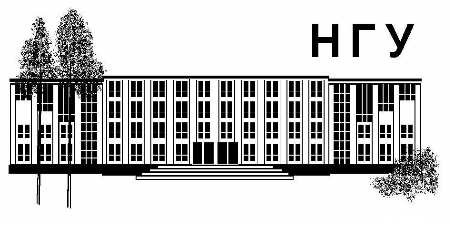
\includegraphics[width=0.18\textwidth]{../NSU-logo}

    Кафедра теоретической физики физического факультета НГУ

    \large
    Профессор Фадин В.\,С.
    \vspace{-0.5em}

    \huge
    \textbf{Теория сильных взаимодействий}
    
    \Large
    Лекция № 13
    \vfill
    
    \normalsize
    \begin{minipage}{0.95\linewidth}
      \small Дисперсионное правило сумм для распада $J/\psi$"=мезона:
      дисперсионные интегралы $A_n$, приближение узких резонансов,
      нахождение ширины распада $J/\psi$ в $e^+e^-$. Проблемы для
      $A_n$ при больших $n$. Необходимость введения глюонного
      конденсата и его вклад в $A_n$. Пропагатор кварка в фоновом
      поле. Ренорм-инвариантность
      $\alpha_s\left(G^a_{\mu\nu}\right)^2$. Правила сумм для
      $\rho$"=мезонов. Изовекторный ток. Вклад в поляризационный оператор
      глюонного и кваркового конденсатов. Спонтанное нарушение
      симметрии. Теорема Голдстоуна. Спонтанное нарушение непрерывных
      симметрий. Механизм Хиггса. Киральная симметрия безмассового
      лагранжиана КХД. Псевдоголдстоуновские бозоны. Киральный
      (аксиальный) ток. Нуклонные матричные элементы кирального
      тока. Нуклонные матричные элементы аксиального тока: формфакторы
      $g_a$, $h_a$. Иллюстрация теоремы Голдстоуна: наличие $\pi$"=мезонного
      полюса в формфакторе $h_a$.
    \end{minipage}
    \vfill
    
    \normalsize \ccbysa\hspace{0.5em} Новосибирск 2014   
  \end{center}
\end{titlepage}
\end{document}
